\subsection{Fundamentals of NS theory}\label{NS Fundamentals} Software architectures
should be able to evolve as business requirements change over time. In NS theory,
evolvability is measured by the lack of Combinatorial Effects. When the impact of a change
depends not only on the type of the change but also on the size of the system it affects,
we talk about a Combinatorial Effect. The NS theory assumes that software undergoes
unlimited evolution (i.e., new and changed requirements over time, so Combinatorial
Effects are very harmful to software evolvability. Indeed, suppose changes to a system
depend on the size of the growing system. In that case, these changes become more
challenging to handle (i.e., requiring more work and lowering the system's evolvability. 

NS theory is built on classic system engineering and statistical entropy principles. In
classic system engineering, a system is stable if it has BIBO – Bounded Input leading to
Bounded Output. NS theory applies this idea to software design as a limited change in
functionality should cause a limited change in the software. In classic system
engineering, stability is measured at infinity. NS theory considers infinitely large
systems that will go through infinitely many changes. A system is stable for NS, if it
does not have CE, meaning that the effect of change only depends on the kind of change and
not on the system size.

NS theory suggests four theorems and five extendable elements as the basis for creating
evolvable software through pattern expansion of the elements. The theorems are proved
formally, and they give a set of required conditions that must be followed strictly to
avoid Combinatorial Effects. The NS theorems have been applied in NS elements. These
elements offer a set of predefined higher-level structures, patterns, or “building blocks”
that provide a clear blueprint for implementing the core functionalities of realistic
information systems, following the four theorems.
%
% 1.2.1 NS Theorems
%
\subsubsection{NS Theorems}\label{NS Theorems}
NS theory proposes four theorems, which have been proven, to dictate the necessary conditions for software to be free of Combinatorial Effects.
\begin{itemize}
    \item Separation of Concerns 
    \item Data Version Transparency
    \item Action Version Transparency 
    \item Separation of States
\end{itemize}
Violation of any of these 4 theorems will lead to Combinatorial Effects and, thus, non-evolvable software under change.
%
% 1.2.2 NS Elements
%
\subsubsection{NS Elements}\label{NS Elements} Consistently adhering to the four NS
theorems is very challenging for developers. First, following the NS theorems leads to a
fine-grained software structure. Creating such a structure introduces some development
overhead that may slow the development process. Secondly, the rules must be followed
constantly and robotically, as a violation will introduce Combinatorial Effects. Humans
are not well suited for this kind of work. Thirdly, the accidental introduction of
Combinatorial Effects results in an exponential increase of rework that needs to be done.

Five expandable elements—data, action, workflow, connector, and trigger — were proposed to
make the realization of NS applications more feasible. These carefully engineered patterns
comply with the four NS theorems and can be used as essential building blocks for a wide
variety of applications.

\begin{itemize}
    \item \textbf{Data Element}: the structured composition of software constructs to encapsulate a data construct into an isolated module (including get- and set methods, persistency, exhibiting version transparency,etc.).
    \item \textbf{Action Elements}: the structured composition of software constructs to encapsulate an action construct into an isolated module.
    \item \textbf{Workflow Element}: the structured composition of software constructs describing the sequence in which action elements should be performed to fulfil a flow into an isolated module.
    \item \textbf{Connector Element}: the structured composition of software constructs into an isolated module, allowing external systems to interact with the NS system without statelessly calling components.
    \item \textbf{Trigger Element}: the structured composition of software constructs into an isolated module that controls the system states and checks whether any action element should be triggered accordingly.
\end{itemize}

The element provides core functionalities (data, actions, etc.) and addresses the
cross-cutting concerns that each core functionality requires to function properly. As
cross-cutting concerns cut through every element, they require careful implementation to
avoid introducing Combinatorial Effects.
%
% 1.2.3 Element Expansion
%
\subsubsection{Element Expansion}\label{Element Expansion} An application is composed of a
set of data, action, workflow, connector, and trigger elements that define its
requirements. The NS expander is a technology that will generate code instances of
high-level patterns for the specific application. The expanded code will provide generic
functionalities specified in the application definition and will be a fine-grained modular
structure that follows the NS theorems (see Figure~\ref{fig_1}).

The application's business logic is now manually programmed inside the expanded modules at
pre-defined locations. The result is an application that implements a certain required
business logic and has a fine-grained modular structure. As the code's generated structure
is NS compliant, we know that the code is evolvable for all anticipated change drivers
corresponding to the underlying NS elements. The only location where Combinatorial Effects
can be introduced is in the customized code.
\begin{figure}[htbp]
\centering
\centerline{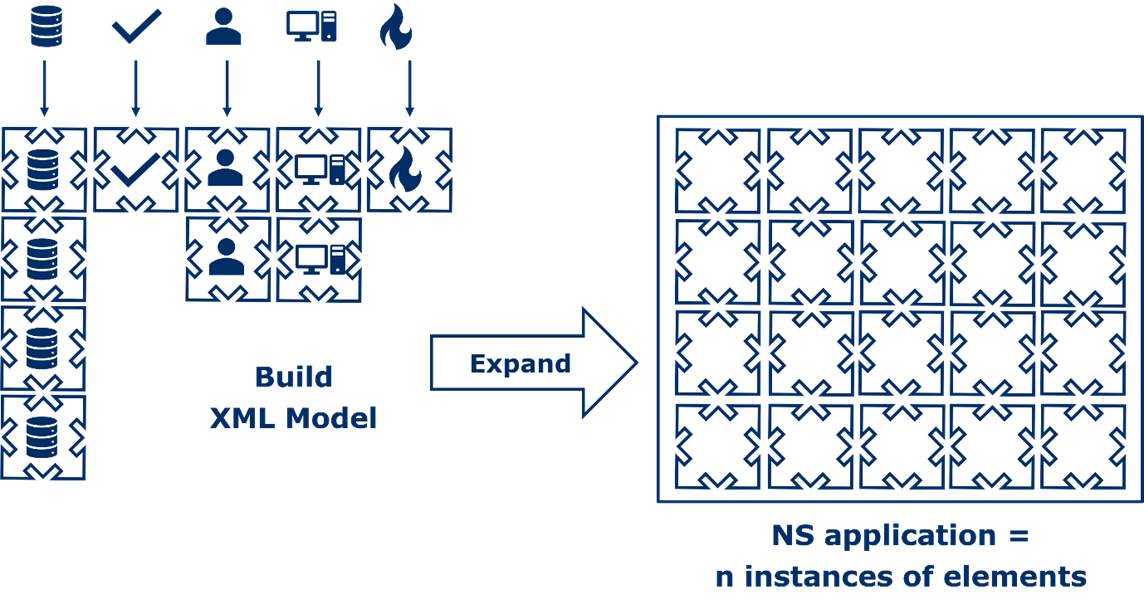
\includegraphics[scale=0.7]{figures/Picture1.png}}
\caption{Requirements expressed in XML description file, used on input for element expansion.}
\label{fig_1}
\end{figure}

%
% 1.2.4 Harvesting and Software Rejuvenation
%
\subsubsection{Harvesting and Software Rejuvenation}\label{Harvesting and Software
Rejuvenation} The expanded code has some pre-defined places where changes can be made. To
prevent these changes from being lost when the application is expanded again, the expander
can gather them and return them when it is re-expanded. Gathering and returning the
changes is called harvesting and injection.

The application can be re-expanded for different reasons. For example, the code templates
of the elements are improved (fix bugs, make faster, etc., include a new cross-cutting
concern (add a new logging feature, or change the technology (use a new persistence
framework.

Software rejuvenation aims to routinely carry out the harvesting and injection process to
ensure that the constant enhancements to the element code templates are incorporated into
the application.

Code expansion produces more than 80\% of the code of the application. The expanded code
can be called boiler-plate-code, but it is more complex than what is usually meant by that
term because it deals with Cross-Cutting Concerns. Manually producing this code takes a
lot of time. Using NS expansion, this time can now be spent on the constant improvement of
the code templates, the development of new code templates that make the elements
compatible with the latest technologies, and the meticulous coding of the business logic.
The changes in the elements can be applied to all expanded applications, giving the
concept of code reuse a new meaning. All developers can use a modification on a code
template by one developer on all their applications with minimal impact, thanks to the
rejuvenation process. Figure~\ref{fig_2} summarizes the NS development process.
\begin{figure}[htbp]
\centering
\centerline{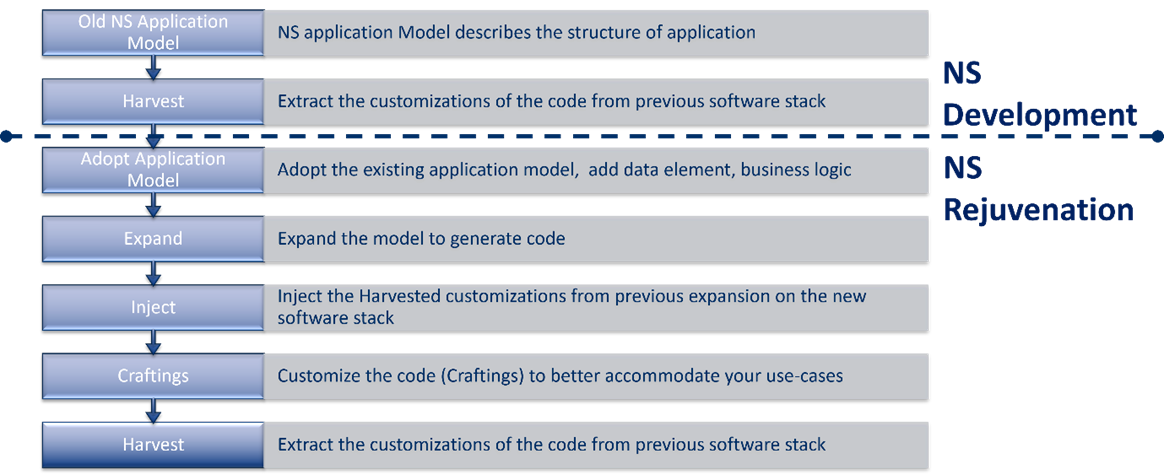
\includegraphics[scale=0.65]{figures/Picture2.png}}
\caption{The NS development process.}
\label{fig_2}
\end{figure}
%
% 1.2.5 Dimensions of Change
%
\subsubsection{Dimensions of Change}\label{Dimensions of Change} Element expansion,
harvesting, rejuvenation and injection protect against CE from four change dimensions. The
first dimension is the addition of new instances of data, task, flow, trigger and
connector elements. These types of changes originate from new functionalities. The second
dimension is the changes to the element code templates due to the introduction of new
cross-cutting concerns or the overall improvement of the code of the templates. The third
dimension is technology-induced changes, handled by the cross-cutting concerns and thus
via the element templates. The fourth and last dimension represents the custom code, the
crafting, which can be harvested and reinjected.
